% Author : Alain Matthes
% Encoding : UTF8
% Engine : PDFLaTeX
\documentclass[]{article}
\usepackage[utf8]{inputenc} 
\usepackage[usenames,dvipsnames]{xcolor}
\usepackage{fullpage}
\usepackage[upright]{fourier}
\usepackage{tkz-graph}
\thispagestyle{empty}
\begin{document}
\begin{center}
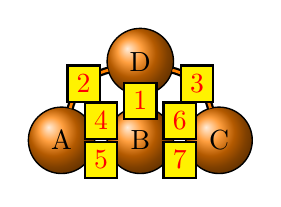
\begin{tikzpicture}[node distance   = 4 cm]
     \GraphInit[vstyle=Shade]
     \tikzset{LabelStyle/.style =   {draw,
                                     fill  = yellow,
                                     text  = red}}
     \Vertex{A}
     \EA(A){B}
     \EA(B){C}
     \tikzset{node distance   = 8 cm}% modifie la distance entre les nodes
     \NO(B){D}
     \Edge[label=1](B)(D)
     \tikzset{EdgeStyle/.append style = {bend left}}
     \Edge[label=4](A)(B)
     \Edge[label=5](B)(A)
     \Edge[label=6](B)(C)
     \Edge[label=7](C)(B)
     \Edge[label=2](A)(D)
     \Edge[label=3](D)(C)
  \end{tikzpicture}
\end{center}
\end{document}
